\newpage

\begin{lstlisting}[language=JuliaLocal, style=julia]
using PlutoUI
\end{lstlisting}

\begin{lstlisting}[language=JuliaLocal, style=julia]
begin
	using Plots
	y(x) = sin(x)
	plot(y,
		color=:blue)
end
\end{lstlisting}

\begin{figure}[H]
	\centering
	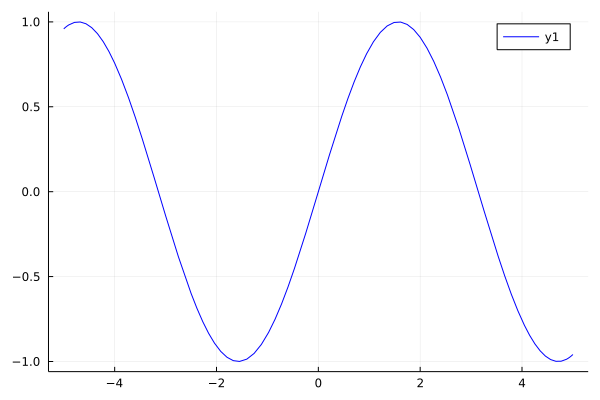
\includegraphics[width=0.8\textwidth]{./figures/examplepluto_figure1.png}
	\label{fig:examplepluto_figure1.png}

\end{figure}

\begin{lstlisting}[language=JuliaLocal, style=julia]
A = [10,10,10]
\end{lstlisting}

\begin{verbatim}
3-element Vector{Int64}:
 10
 10
 10
\end{verbatim}

\begin{lstlisting}[language=JuliaLocal, style=julia]
x = rand(10);
\end{lstlisting}

\begin{lstlisting}[language=JuliaLocal, style=julia]
x .+ 1
\end{lstlisting}

\begin{verbatim}
10-element Vector{Float64}:
 1.7628714129957028
 1.3555389111225373
 1.4291094785319325
 1.9961534157731415
 1.5140054961259364
 1.2228365779406158
 1.0961750891793673
 1.7292439442049676
 1.9921209010034493
 1.2256276790206206
\end{verbatim}

\begin{lstlisting}[language=JuliaLocal, style=julia]
set_theme!(theme_ggplot2())
\end{lstlisting}

\begin{lstlisting}[language=JuliaLocal, style=julia]
Makie.plot(x)
\end{lstlisting}

\begin{figure}[H]
	\centering
	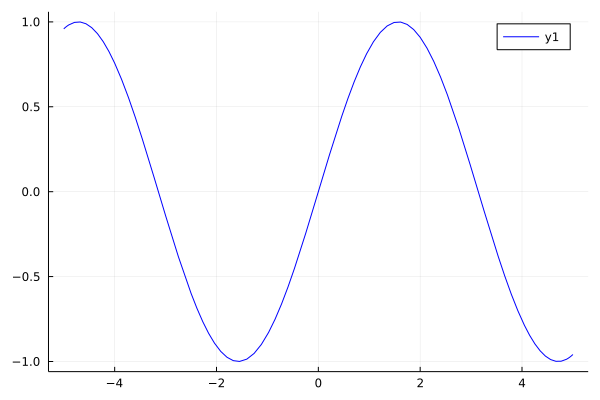
\includegraphics[width=0.8\textwidth]{./figures/examplepluto_figure2.png}
	\label{fig:examplepluto_figure2.png}

\end{figure}

\begin{lstlisting}[language=JuliaLocal, style=julia]
PlutoUI.LocalResource("figure.svg")
\end{lstlisting}

\begin{lstlisting}[language=JuliaLocal, style=julia]
PlutoUI.LocalResource(figurepath)
\end{lstlisting}
